% !TEX root = ../thesis-example-en.tex
\chapter{Probing 2D Superconductivity}\label{sec:fabrication}

\section{Introduction}

\section{2D superconductivity}

\section{Pearl model}

\section{Scanning Quantum Microscopy}

\subsection{Mapping Meissner effect and vortices}

Local magnetic field measurements are performed on thin-layer samples of the two-dimensional superconductor 2H-\ce{NbSe2} utilizing the developed cryogenic atomic force microscope (AFM) and magnetometer, operating at a base temperature of 1.8 K. The sample investigated is as depicted in \cref{fig:s2_ovw}. The different large flake of the material also has two thicker regions towards the edge, visible as different contrast in the micrograph. The AFM scan shows the presence of bubbles and residue that is inherent to the vdW material transfer process used, rendering a challenging landscape for most scanning probes.

A single Nitrogen-Vacancy (NV) center, facilitates the detection of local magnetic responses from the \ce{NbSe2} sample, through the protective hexagonal boron nitride \ce{h-BN} cladding. The \ce{NbSe2} two distinct thickness regions in th flake are: $\qty{5.03}{\nano\meter}$ (corresponding to seven atomic layers) and $\qty{12.55}{\nano\meter}$. 

\begin{figure}[H]
    \centering 
    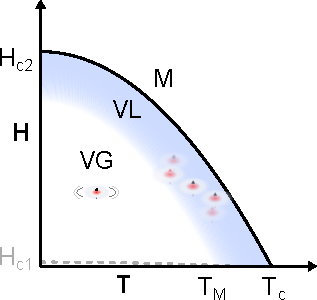
\includegraphics[width=0.5\textwidth]{../figures/phase_diag.pdf}
    \caption{Phase diagram of few layer \ce{NbSe2} flake as a function of temperature and magnetic field, identifying three distinct phases: vortex glass, vortex liquid, and a metallic state.}
    \label{fig:phase_diag}
\end{figure}

The phase diagram for the thinner \ce{NbSe2} region, illustrated in \cref{fig:phase_diag}, delineates three distinct regimes: the vortex glass (VG), vortex liquid (VL), and metallic (M) states. These phases were identified via transport measurements characterizing the transitions between superconducting and dissipative states\cite{zhangNonreciprocalSuperconductingNbSe22020}. In this context, $T_M$ denotes the melting temperature, while $H_{c1}$ and $H_{c2}$ correspond to the lower and upper critical fields of a type-II superconductor, respectively.

\cref{fig:s2_ovw} displays a magnetic scan acquired at the metallic phase and at \qty{2}{\kelvin}, within the vortex glass state. The data reveals a pronounced diamagnetic response along the flake edge, indicative of the Meissner effect. Control measurements taken at \qty{10}{\kelvin} ($T > T_c$) show a complete vanishing of this magnetic response, confirming that the signals observed at \qty{2}{\kelvin} originate exclusively from the superconducting state.

\begin{figure}[H]
    \centering 
    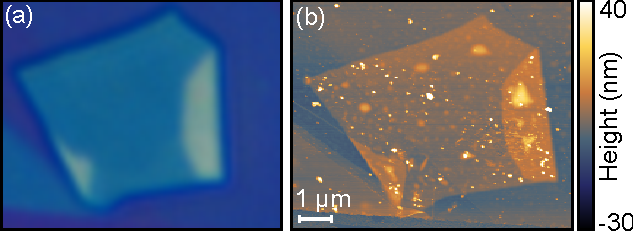
\includegraphics[width=\textwidth]{../figures/sample_s2_ovw.pdf}
    \caption{(a) Optical micrograph of 2H-\ce{NbSe2} sample S2. The brighter regions are thicker than the rest of the flake. 
    (b) An AFM scan of the flake. The large flake area is $\qty{5.03}{\nano\meter}$ thick, and the 
    thicker region on the right side of the flake is $\qty{12.55}{\nano\meter}$ thick.}
    \label{fig:s2_ovw}
\end{figure}

Due to the geometric confinement of the sample, where the flake thickness is significantly less than the London penetration depth of bulk \ce{NbSe2} ($\lambda \approx \qty{125}{\nano\meter}$)\cite{callaghanFieldDependenceVortex2005,fletcherPenetrationDepthStudy2007}, the external magnetic field is only partially screened. The effective field screening is approximately \qty{-100}{\micro\tesla}. 

Superimposed on this background, positive magnetic signals are observed and attributed to superconducting vortices, which persist across the majority of the superconducting phase space. Notably, vortex nucleation occurs at external field strengths as low as a few \unit{\milli\tesla}, a value significantly below the first critical field ($H_{c1}$) reported for bulk \ce{NbSe2}.

This premature vortex formation is a consequence of the sample's few-layer thickness, which permits magnetic field penetration and local suppression of the superconducting order parameter.

\begin{figure}[H]
    \centering 
    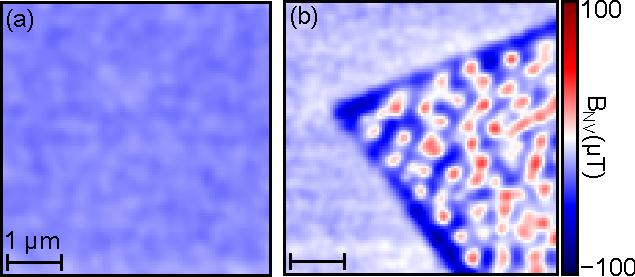
\includegraphics[width=\textwidth]{../figures/vortices_s2.pdf}
    \caption{(a) Magnetometry of the corner of sample S2, at a temperature of \qty{10}{\kelvin}, and a 
    magnetic field of \qty{6}{\milli\tesla} applied out of the plane of the sample. 
    (b) Magnetometry performed at \qty{2.5}{\kelvin}, and identical magnetic field as (a).}
    \label{fig:vortices_s2}
\end{figure}

The vertical confinement inherent to the thin \ce{NbSe2} layers induces a radial expansion of the vortices, consistent with the Pearl vortex model\cite{pearlCURRENTDISTRIBUTIONSUPERCONDUCTING1964}. High-resolution scanning of a single vortex (\cref{fig:s2_single}) confirms this profile; the vortex exhibits a spatial extent exceeding that of bulk vortices, aligning with the scaling behavior predicted for Pearl vortices in thin-film superconductors\cite{fridmanAnomalousThicknessDependence2025}. 

Post-fabrication characterization via AFM (\cref{fig:s2_ovw}) indicates the presence of surface residue on the flake. While such surface contamination presents significant technical impediments for tunneling-based probes like Scanning Tunneling Microscopy (STM)\cite{zomerFastPickTechnique2014}, the Scanning Quantum Microscopy (SQM) technique employed here demonstrates superior robustness. SQM enables high-resolution, non-invasive mapping of superconducting vortices despite surface imperfections. Although residues may induce minor artifacts in the magnetic field map, these deviations are systematically correctable a-posteriori by correlating the magnetic data with AFM topography.

\begin{figure}[H]
    \centering 
    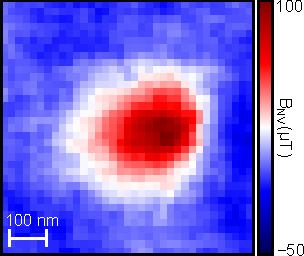
\includegraphics[width=0.5\textwidth]{../figures/single_vortex.pdf}
    \caption{High-resolution scan resolving a single vortex in the 2H-\ce{NbSe2} flake.}
    \label{fig:s2_single}
\end{figure}

In the regime of few-layer \ce{NbSe2}, the superconducting response is strongly influenced by substrate roughness, structural disorder, and finite-size effects. These local perturbations induce significant deviations from the canonical vortex profile and arrangements typically observed in pristine superconductors, resulting in distorted and anisotropic vortex cores. Furthermore, the multi-band nature of superconductivity in \ce{NbSe2}\cite{noatQuasiparticleSpectra22015,zehetmayerExperimentalEvidenceTwoband2010} allows for the potential stabilization of multi-flux-quanta vortices\cite{gozlinskiBandresolvedCaroliGennes2023}.

% Figure 2(a) presents a representative magnetic field distribution for the thin sample, where a coherent hexagonal vortex lattice is notably absent. This lack of long-range order is quantified via autocorrelation analysis in Fig. 2(b), which exhibits elongated and irregular correlation peaks. While a nascent hexagonal symmetry is faintly discernible, the arrangement is heavily obscured by disorder. As corroborated by Fig. S5 in the Supplemental Material [35], the vortex lattice topology is strongly rectified by the sample boundary, with autocorrelation features aligning along the geometric edges. Although hexagonal ordering becomes more pronounced toward the sample center, local disorder remains the dominant energetic constraint, preventing the formation of a perfect Abrikosov lattice.X.5.2 Vortex Dynamics and DelocalizationAt temperatures significantly below $T_c$, the magnetic imaging reveals anisotropic, line-shaped structures (Fig. 2(a)). We attribute these features not to static deformations, but to the rapid spatial fluctuation of circular vortices between metastable pinning sites. This quasi-delocalization effectively integrates to an elongated signal within the SQM measurement window. Such dynamics are likely driven by the interplay between the underlying potential landscape (disorder) and the enhanced thermal fluctuations characteristic of 2D superconductors [45].X.5.3 Comparative Analysis of Lattice SymmetryTo isolate the effects of dimensionality and surface quality, comparative measurements were performed on a thicker (> 10 nm) \ce{NbSe2} sample (S2), fully encapsulated in h-BN to preserve interface integrity (see Fig. S2 in Supplemental Material [35]). In this regime, the vortex matter crystallizes into a distinct Abrikosov lattice, exhibiting long-range hexagonal order across the majority of the scan area [Fig. 2(c)]. The corresponding autocorrelation analysis [Fig. 2(d)] confirms this structural recovery, though minor distortions persist, arising from the competition between elastic lattice forces, geometric confinement, and residual spatial disorder.X.5.4 Implications for Transport PhenomenaIt is pertinent to note that the deviation from hexagonal symmetry in the thin-film limit has profound implications for the interpretation of macroscopic transport experiments. The frequent assumption of a pristine lattice in such systems is often invalid. Consequently, characterizing the specific, non-hexagonal vortex arrangement is essential for the accurate deduction of the superconducting ground state symmetry from transport data.

\begin{figure}[H]
    \centering 
    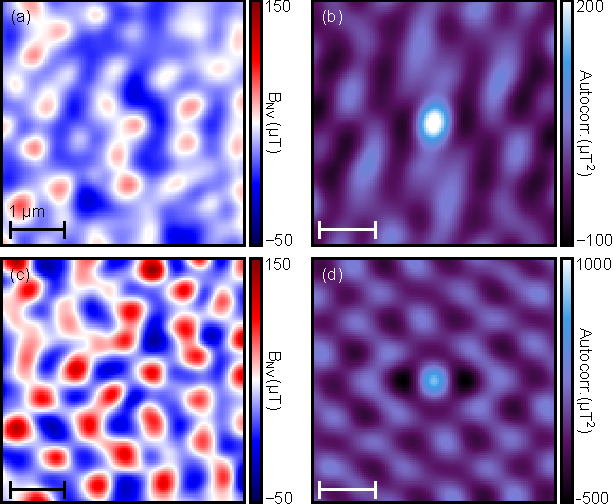
\includegraphics[width=\textwidth]{../figures/thick_thin.pdf}
    \caption{Vortex arrangements in \ce{NbSe2} with varying thickness. 
    (a),(b) Magnetic field map and corresponding autocorrelation of a thin $\qty{5.03}{\nano\meter}$ sample, on an oxide 
    substrate and encapsulated with \ce{h-BN}. The vortex configuration appears disordered, showing weak spatial 
    correlations and broad, smeared autocorrelation peaks. (c),(d) Magnetic field map and autocorrelation of a 
    thicker, $\qty{11.59}{\nano\meter}$ \ce{NbSe2} sample, fully encapsulated with h-BN, revealing enhanced vortex hexagonal ordering. 
    All scale bars are $\qty{1}{\micro\meter}$.}
    \label{fig:thick_thin}
\end{figure}

\begin{figure}[H]
    \centering 
    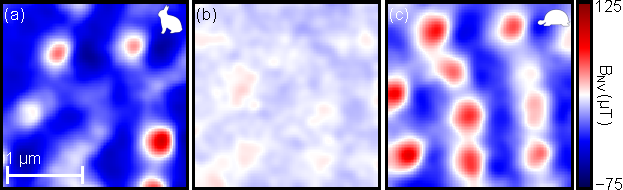
\includegraphics[width=\textwidth]{../figures/fast_slow.pdf}
    \caption{Cooling-rate-dependent vortex arrangements in a $\qty{5.03}{\nano\meter}$ \ce{NbSe2} sample.
    (a) SQM magnetometry of a thin \ce{NbSe2} flake after rapid cooling (from \qty{6.3}{\kelvin} to \qty{3.9}{\kelvin} within \qty{1}{\minute}), 
    showing weak magnetic contrast. (b) Magnetic field map of the same region at \qty{6.3}{\kelvin}. (c) Magnetic field map after 
    slow cooling (from \qty{6.3}{\kelvin} to \qty{1.9}{\kelvin} over several hours), showing enhanced vortex contrast, and rearrangement. 
    Scale bar is $\qty{1}{\micro\meter}$.}
    \label{fig:fast_slow}
\end{figure}
